\documentclass[border=5pt]{standalone}
\usepackage{tikz}
\usepackage{amsmath}
\usepackage{amssymb}
\usepackage{bm}
\usetikzlibrary{positioning, arrows.meta, calc, fit, backgrounds, shapes.geometric}

% Blue-Gray academic scheme
\definecolor{bgPrimary}{HTML}{DAE8FC}
\definecolor{bgSecondary}{HTML}{E8EEF7}
\definecolor{bgAccent}{HTML}{B3CDE3}
\definecolor{bgInput}{HTML}{F0F4F8}
\definecolor{borderPrimary}{HTML}{6C8EBF}
\definecolor{borderAccent}{HTML}{3A6EA5}
\definecolor{arrowColor}{HTML}{4A6A8A}
\definecolor{textMain}{HTML}{2C3E50}
\definecolor{textLight}{HTML}{7F8C8D}
\definecolor{bgHighlight}{HTML}{FFF3CD}
\definecolor{borderHighlight}{HTML}{C9A227}
\definecolor{bgTree}{HTML}{FDEBD0}
\definecolor{borderTree}{HTML}{CA6F1E}

\tikzset{
  module/.style={draw=borderPrimary, fill=bgPrimary, rounded corners=4pt,
    minimum width=2.5cm, minimum height=1.15cm, font=\sffamily\footnotesize,
    text=textMain, line width=0.6pt, align=center},
  novelmodule/.style={draw=borderAccent, fill=bgAccent, rounded corners=4pt,
    minimum width=2.5cm, minimum height=1.15cm, font=\sffamily\footnotesize,
    text=textMain, line width=1.0pt, align=center},
  treemodule/.style={draw=borderTree, fill=bgTree, rounded corners=4pt,
    minimum width=2.5cm, minimum height=1.15cm, font=\sffamily\footnotesize,
    text=textMain, line width=0.6pt, align=center},
  iobox/.style={draw=borderPrimary, fill=bgInput, rounded corners=3pt,
    minimum width=2.5cm, minimum height=1.05cm, font=\sffamily\footnotesize,
    text=textMain, line width=0.5pt, align=center},
  outbox/.style={draw=borderAccent, fill=bgHighlight, rounded corners=3pt,
    minimum width=2.6cm, minimum height=1.0cm, font=\sffamily\footnotesize,
    text=textMain, line width=0.8pt, align=center},
  fuse/.style={draw=borderAccent, fill=bgAccent, circle, minimum size=0.72cm,
    font=\sffamily\small\bfseries, text=textMain, line width=1.0pt, inner sep=1pt},
  stdarrow/.style={-{Stealth[length=2.6mm]}, line width=0.75pt, color=arrowColor},
  dasharrow/.style={-{Stealth[length=2.6mm]}, line width=0.7pt, color=arrowColor, dashed},
  albl/.style={font=\sffamily\scriptsize, text=textLight, fill=white, inner sep=1pt},
  grouptitle/.style={font=\sffamily\small\bfseries, text=textMain},
}

\begin{document}
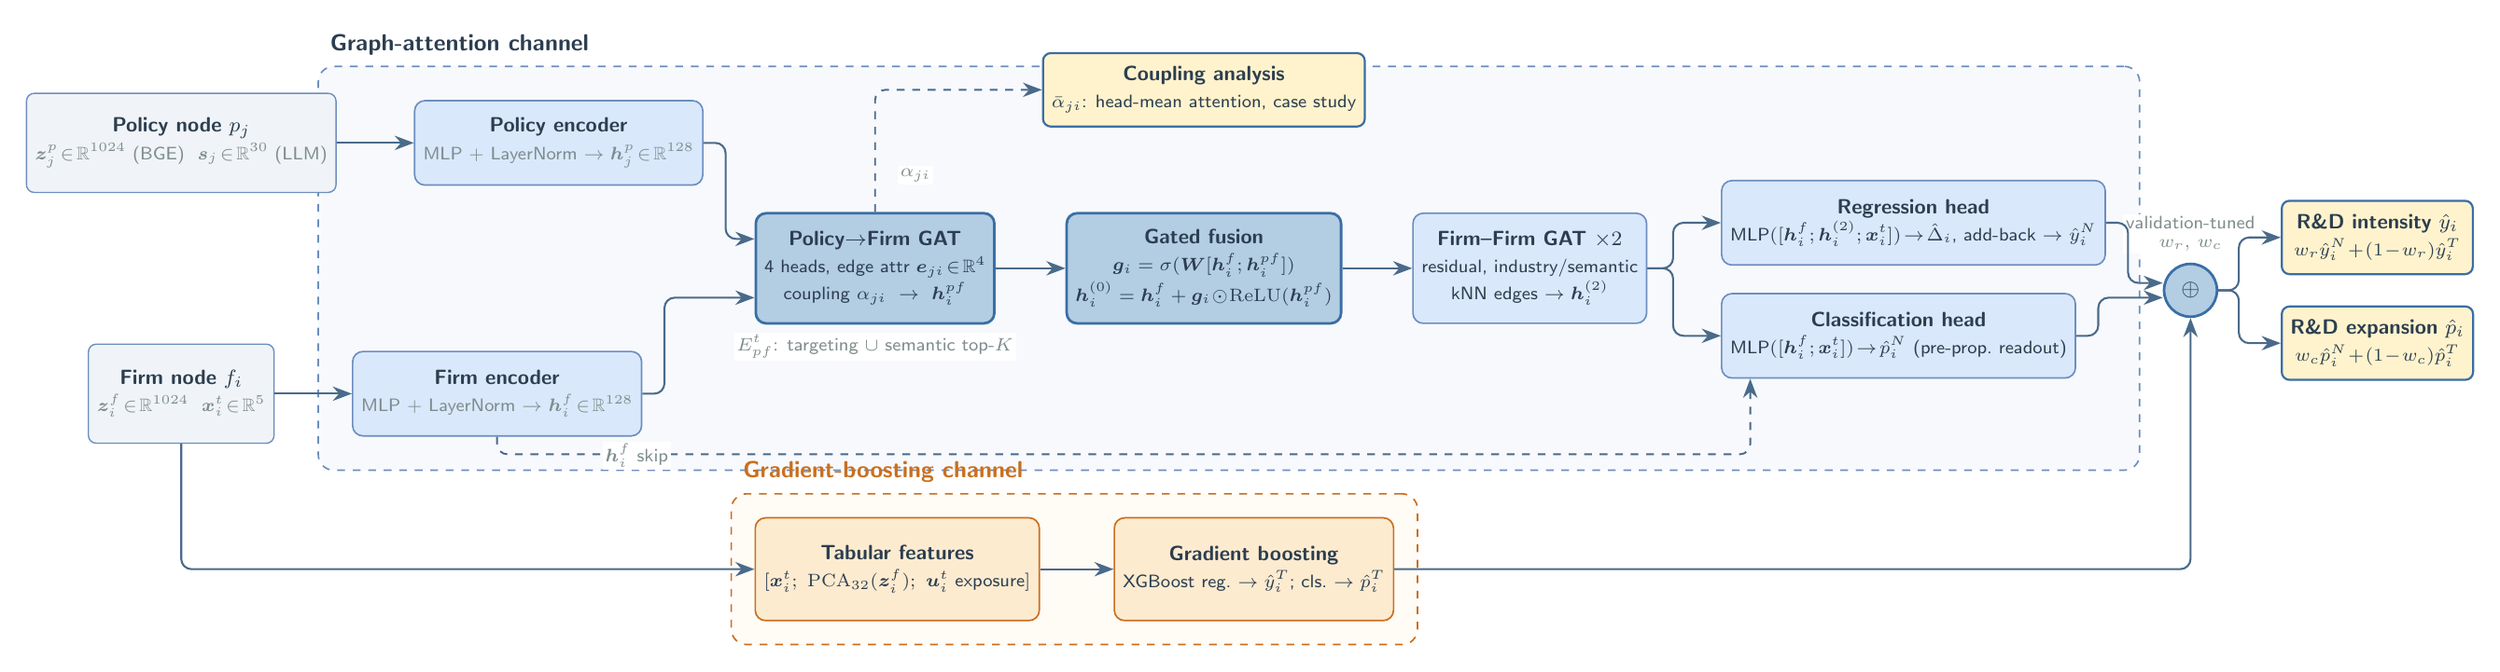
\begin{tikzpicture}[node distance=0.85cm]

% ---------- inputs ----------
\node[iobox, minimum height=1.35cm] (pin) {\textbf{Policy node} $p_j$\\[1pt]
  {\scriptsize\color{textLight}$\bm{z}_j^{p}\!\in\!\mathbb{R}^{1024}$ (BGE)\ \ $\bm{s}_j\!\in\!\mathbb{R}^{30}$ (LLM)}};
\node[iobox, minimum height=1.35cm, below=2.05cm of pin] (fin) {\textbf{Firm node} $f_i$\\[1pt]
  {\scriptsize\color{textLight}$\bm{z}_i^{f}\!\in\!\mathbb{R}^{1024}$\ \ $\bm{x}_i^{t}\!\in\!\mathbb{R}^{5}$}};

% ---------- neural channel ----------
\node[module, right=1.05cm of pin] (penc) {\textbf{Policy encoder}\\[1pt]
  {\scriptsize\color{textLight}MLP + LayerNorm $\rightarrow \bm{h}_j^{p}\!\in\!\mathbb{R}^{128}$}};
\node[module, right=1.05cm of fin] (fenc) {\textbf{Firm encoder}\\[1pt]
  {\scriptsize\color{textLight}MLP + LayerNorm $\rightarrow \bm{h}_i^{f}\!\in\!\mathbb{R}^{128}$}};

\node[novelmodule, minimum height=1.5cm] (gat) at ($(penc.east)!0.5!(fenc.east) + (2.75cm,0)$)
  {\textbf{Policy$\rightarrow$Firm GAT}\\[1pt]
  {\scriptsize 4 heads, edge attr $\bm{e}_{ji}\!\in\!\mathbb{R}^{4}$}\\[1pt]
  {\scriptsize coupling $\alpha_{ji}\ \rightarrow\ \bm{h}_i^{pf}$}};

\node[novelmodule, right=0.95cm of gat, minimum height=1.5cm] (gate)
  {\textbf{Gated fusion}\\[1pt]
  {\scriptsize $\bm{g}_i=\sigma(\bm{W}[\bm{h}_i^{f};\bm{h}_i^{pf}])$}\\[1pt]
  {\scriptsize $\bm{h}_i^{(0)}=\bm{h}_i^{f}+\bm{g}_i\!\odot\!\mathrm{ReLU}(\bm{h}_i^{pf})$}};

\node[module, right=0.95cm of gate, minimum height=1.5cm] (ffgat)
  {\textbf{Firm--Firm GAT $\times 2$}\\[1pt]
  {\scriptsize residual, industry/semantic}\\[1pt]
  {\scriptsize kNN edges $\rightarrow \bm{h}_i^{(2)}$}};

% heads
\node[module, right=1.0cm of ffgat, yshift=0.62cm, minimum width=3.0cm] (reghead)
  {\textbf{Regression head}\\[1pt]
  {\scriptsize MLP$([\bm{h}_i^{f};\bm{h}_i^{(2)};\bm{x}_i^{t}])\!\rightarrow\!\hat{\Delta}_i$, add-back $\rightarrow \hat{y}_i^{N}$}};
\node[module, right=1.0cm of ffgat, yshift=-0.92cm, minimum width=3.0cm] (clshead)
  {\textbf{Classification head}\\[1pt]
  {\scriptsize MLP$([\bm{h}_i^{f};\bm{x}_i^{t}])\!\rightarrow\!\hat{p}_i^{N}$ (pre-prop.\ readout)}};

% ---------- coupling output ----------
\node[outbox, above=1.15cm of gate, minimum width=3.1cm] (coup)
  {\textbf{Coupling analysis}\\[1pt]{\scriptsize $\bar{\alpha}_{ji}$: head-mean attention, case study}};

% ---------- tree channel ----------
\node[treemodule, minimum width=3.4cm, minimum height=1.4cm, below=4.1cm of gat.west, anchor=west]
  (feat) {\textbf{Tabular features}\\[1pt]
  {\scriptsize $[\bm{x}_i^{t};\ \mathrm{PCA}_{32}(\bm{z}_i^{f});\ \bm{u}_i^{t}\ \text{exposure}]$}};
\node[treemodule, right=1.0cm of feat, minimum width=3.2cm, minimum height=1.4cm] (xgb)
  {\textbf{Gradient boosting}\\[1pt]
  {\scriptsize XGBoost reg.\ $\rightarrow\hat{y}_i^{T}$;\ cls.\ $\rightarrow\hat{p}_i^{T}$}};

% ---------- fusion + outputs ----------
\node[fuse] (fusion) at ($(reghead.east) + (1.15cm, -0.92cm)$) {$\oplus$};
\node[albl, above=0.12cm of fusion, align=center] {validation-tuned\\[-1pt]$w_r,\,w_c$};

\node[outbox, right=0.85cm of fusion, yshift=0.72cm] (out1)
  {\textbf{R\&D intensity} $\hat{y}_i$\\[1pt]{\scriptsize $w_r\hat{y}_i^{N}\!+\!(1\!-\!w_r)\hat{y}_i^{T}$}};
\node[outbox, right=0.85cm of fusion, yshift=-0.72cm] (out2)
  {\textbf{R\&D expansion} $\hat{p}_i$\\[1pt]{\scriptsize $w_c\hat{p}_i^{N}\!+\!(1\!-\!w_c)\hat{p}_i^{T}$}};

% ---------- group boxes ----------
\begin{scope}[on background layer]
\node[draw=borderPrimary, dashed, rounded corners=6pt, line width=0.6pt,
      fill=bgSecondary, fill opacity=0.35, inner sep=13pt,
      fit=(penc)(fenc)(gat)(gate)(ffgat)(reghead)(clshead)] (neuralbox) {};
\node[draw=borderTree, dashed, rounded corners=6pt, line width=0.6pt,
      fill=bgTree, fill opacity=0.22, inner sep=9pt,
      fit=(feat)(xgb)] (treebox) {};
\end{scope}
\node[grouptitle, anchor=south west] at ($(neuralbox.north west)+(0.05,0.02)$) {Graph-attention channel};
\node[grouptitle, anchor=south west, text=borderTree] at ($(treebox.north west)+(0.05,0.02)$) {Gradient-boosting channel};

% ---------- arrows ----------
\draw[stdarrow] (pin) -- (penc);
\draw[stdarrow] (fin) -- (fenc);
\draw[stdarrow, rounded corners=4pt] (penc.east) -- ++(0.3,0) |- ($(gat.west)+(0,0.4)$);
\draw[stdarrow, rounded corners=4pt] (fenc.east) -- ++(0.3,0) |- ($(gat.west)+(0,-0.4)$);
\draw[stdarrow] (gat) -- (gate);
\draw[stdarrow] (gate) -- (ffgat);
\draw[stdarrow, rounded corners=4pt] (ffgat.east) -- ++(0.35,0) |- (reghead.west);
\draw[stdarrow, rounded corners=4pt] (ffgat.east) -- ++(0.35,0) |- (clshead.west);
% skip connection h_f to cls head
\draw[dasharrow, rounded corners=4pt]
  (fenc.south) -- ++(0,-0.24) -| ($(clshead.south west)+(0.4,0)$);
\node[albl] at ($(fenc.south)+(1.9,-0.26)$) {$\bm{h}_i^{f}$ skip};
% alpha to coupling
\draw[dasharrow, rounded corners=4pt] (gat.north) |- (coup.west);
\node[albl] at ($(gat.north)+(0.55,0.5)$) {$\alpha_{ji}$};
% tree channel inputs
\draw[stdarrow, rounded corners=4pt] (fin.south) -- ++(0,-0.55) |- (feat.west);
\draw[stdarrow] (feat) -- (xgb);
% edge attr note into gat
\node[albl, align=center] at ($(gat.south)+(0,-0.30)$) {$E_{pf}^{t}$: targeting $\cup$ semantic top-$K$};
% heads to fusion
\draw[stdarrow, rounded corners=4pt] (reghead.east) -- ++(0.3,0) |- ($(fusion.west)+(0,0.1)$);
\draw[stdarrow, rounded corners=4pt] (clshead.east) -- ++(0.3,0) |- ($(fusion.west)+(0,-0.1)$);
% tree to fusion
\draw[stdarrow, rounded corners=4pt] (xgb.east) -- ++(0.4,0) -| (fusion.south);
% fusion to outputs
\draw[stdarrow, rounded corners=4pt] (fusion.east) -- ++(0.28,0) |- (out1.west);
\draw[stdarrow, rounded corners=4pt] (fusion.east) -- ++(0.28,0) |- (out2.west);

\end{tikzpicture}
\end{document}
